\section{Methodology}
\label{sec:methodology}

\subsection{Evaluation Framework Architecture}

The SQLclMCP evaluation suite implements a five-component architecture designed for extensibility and reproducibility:

\subsubsection{Database Connection Module}
Manages connections to Oracle Database using the oracledb Python driver with features:
\begin{itemize}
    \item Connection pooling for concurrent query execution
    \item Automatic timeout handling (default 10 seconds)
    \item Transaction isolation level configuration
    \item Error classification (syntax vs. execution errors)
\end{itemize}

\subsubsection{Baseline Test Suite}
Executes hand-written, production-quality SQL queries as ground truth:
\begin{itemize}
    \item Captures full result sets for semantic comparison
    \item Records execution plans via EXPLAIN PLAN
    \item Measures latency with microsecond precision
    \item Validates baseline queries execute without error
\end{itemize}

\subsubsection{MCP Server Integration}
Communicates with MCP HTTP server through REST API:
\begin{itemize}
    \item POST /generate-sql: Converts natural language to SQL
    \item GET /health: Monitors server availability
    \item Timeout handling for generation failures (5 seconds)
    \item Error classification for diagnostic analysis
\end{itemize}

\subsubsection{Semantic Comparison Engine}
Normalizes and compares result sets with sophisticated value handling:
\begin{itemize}
    \item Decimal to float conversion for numeric comparison
    \item ISO 8601 standardization for temporal values
    \item Tuple sorting for order-independent comparison
    \item NULL handling consistent with SQL semantics
\end{itemize}

\subsubsection{Query Plan Analysis Module}
Extracts EXPLAIN PLAN metrics including:
\begin{itemize}
    \item Optimizer Cost (cumulative cost units)
    \item Cardinality Estimate (row count predictions)
    \item Memory Utilization (bytes allocated)
    \item Execution Plan Details (operations, table access methods)
\end{itemize}

\subsection{Query Formulation and Semantic Matching}

\subsubsection{Value Normalization}

We implement comprehensive value normalization to handle datatype differences between baseline and generated queries:

\begin{equation}
\text{normalize}(v) = \begin{cases}
    \text{float}(v) & \text{if } v \in \mathbb{Z} \cup \mathbb{R} \\
    v.isoformat() & \text{if } v \in \text{DateTime} \\
    v.upper() & \text{if } v \in \text{String, case-insensitive} \\
    v & \text{otherwise}
\end{cases}
\end{equation}

\subsubsection{Semantic Equivalence Definition}

Two query results are semantically equivalent if:
\begin{equation}
\text{EQUIVALENT}(Q_1, Q_2) = \text{sorted}(\text{normalize}(R_1)) = \text{sorted}(\text{normalize}(R_2))
\end{equation}

where $R_i$ denotes the result set of query $Q_i$. This definition accounts for:
\begin{itemize}
    \item Order independence (sorting both result sets)
    \item Type equivalence (normalizing values)
    \item Cardinality (must have same row count)
    \item Schema structure (same columns in same order)
\end{itemize}

\subsection{Performance Metrics}

\subsubsection{Semantic Accuracy}

\begin{equation}
\text{Semantic Accuracy} = \frac{|\{q \in Q : \text{EQUIVALENT}(q_{\text{baseline}}, q_{\text{mcp}})\}|}{|Q|} \times 100\%
\end{equation}

\subsubsection{Row Count Accuracy}

\begin{equation}
\text{Row Count Accuracy} = \frac{1}{N}\sum_{i=1}^{N}\mathbb{1}[|R_{\text{baseline}}(q_i)| = |R_{\text{mcp}}(q_i)|]
\end{equation}

\subsubsection{Latency Metrics}

\begin{align}
\text{Baseline Avg} &= \frac{1}{N}\sum_{i=1}^{N}L_{\text{baseline}}(q_i) \\
\text{MCP Avg} &= \frac{1}{M}\sum_{j=1}^{M}L_{\text{mcp}}(q_j) \\
\text{Latency Overhead} &= \frac{\text{MCP Avg} - \text{Baseline Avg}}{\text{Baseline Avg}} \times 100\%
\end{align}

Percentile latencies computed via:
\begin{equation}
L_p = \text{sorted}(L)[p \cdot |L| / 100]
\end{equation}

\subsubsection{Query Plan Deltas}

\begin{align}
\Delta_{\text{cost}} &= \text{Cost}_{\text{MCP}} - \text{Cost}_{\text{baseline}} \\
\Delta_{\text{cardinality}} &= \text{Card}_{\text{MCP}} - \text{Card}_{\text{baseline}} \\
\Delta_{\text{bytes}} &= \text{Bytes}_{\text{MCP}} - \text{Bytes}_{\text{baseline}}
\end{align}

\subsection{Schema Hint Refinement Protocol}

Empirical runs revealed that schema hints are critical for execution success. We formalize this as a two-step protocol:

\paragraph{Step 1: Table Names Only (Insufficient)}
When the LLM prompt includes only table names (e.g., ``REGION, NATION, CUSTOMER, ORDERS, LINEITEM, SUPPLIER, PART, PARTSUPP''), generation succeeds but execution fails. The LLM produces SQL with generic column names (e.g., \texttt{PARTKEY}, \texttt{NATIONKEY}, \texttt{ORDERDATE}, \texttt{SEGMENT}) that do not exist in TPC-H. Oracle returns \texttt{ORA-00904: invalid identifier}, causing execution and EXPLAIN PLAN to fail. Observed: 100\% generation success, 16\% execution success, 84\% ORA-00904 errors.

\paragraph{Step 2: Full TPC-H Column Names (Required)}
The prompt must include actual column names per table, e.g., \texttt{P\_PARTKEY}, \texttt{S\_NATIONKEY}, \texttt{O\_ORDERDATE}, \texttt{C\_MKTSEGMENT}. With explicit schema context, the LLM generates valid Oracle identifiers, execution succeeds, and EXPLAIN PLAN metrics can be computed. This step is required for meaningful evaluation of RQ2 (efficiency) and RQ3 (optimization potential).

\subsection{Evaluation Protocol}

\begin{figure}[h]
\centering
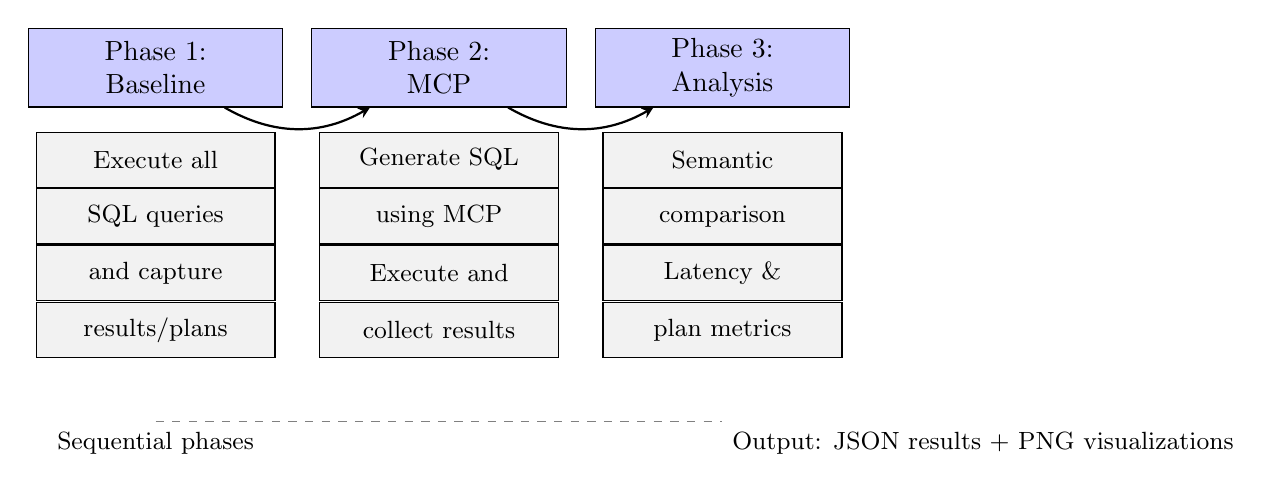
\begin{tikzpicture}[scale=0.9]
  \tikzstyle{phase} = [rectangle, draw, fill=blue!20, text width=3cm, text centered, minimum height=1cm]
  \tikzstyle{arrow} = [thick,->,>=stealth]
  \tikzstyle{detail} = [rectangle, draw, fill=gray!10, text width=2.8cm, text centered, font=\small, minimum height=0.7cm]

  % Phase 1
  \node [phase] (p1) at (0,3) {Phase 1:\\Baseline};
  \node [detail] (p1d1) at (0,1.7) {Execute all};
  \node [detail] (p1d2) at (0,0.9) {SQL queries};
  \node [detail] (p1d3) at (0,0.1) {and capture};
  \node [detail] (p1d4) at (0,-0.7) {results/plans};

  % Phase 2
  \node [phase] (p2) at (4,3) {Phase 2:\\MCP};
  \node [detail] (p2d1) at (4,1.7) {Generate SQL};
  \node [detail] (p2d2) at (4,0.9) {using MCP};
  \node [detail] (p2d3) at (4,0.1) {Execute and};
  \node [detail] (p2d4) at (4,-0.7) {collect results};

  % Phase 3
  \node [phase] (p3) at (8,3) {Phase 3:\\Analysis};
  \node [detail] (p3d1) at (8,1.7) {Semantic};
  \node [detail] (p3d2) at (8,0.9) {comparison};
  \node [detail] (p3d3) at (8,0.1) {Latency \&};
  \node [detail] (p3d4) at (8,-0.7) {plan metrics};

  % Phase arrows
  \draw [arrow] (p1) to[bend right] (p2);
  \draw [arrow] (p2) to[bend right] (p3);

  % Detail arrows
  \draw [arrow, draw=none] (p1) -- (p1d1);
  \draw [arrow, draw=none] (p2) -- (p2d1);
  \draw [arrow, draw=none] (p3) -- (p3d1);

  % Timeline annotation
  \draw [gray, dashed] (0,-2) -- (8,-2);
  \node at (0,-2.3) [font=\small] {Sequential phases};
  \node at (8,-2.3) [font=\small, right] {Output: JSON results + PNG visualizations};
\end{tikzpicture}
\caption{Three-Phase Evaluation Protocol. (1) Baseline phase executes all gold-standard SQL queries and captures row results, execution plans, and latency. (2) MCP phase generates SQL from natural language using Claude API over REST, executes generated queries, and measures MCP latency overhead. (3) Analysis phase performs semantic comparison via normalized tuple sorting and extracts query optimization metrics from EXPLAIN PLAN output.}
\label{fig:evaluation_protocol}
\end{figure}


The evaluation follows a three-phase protocol implemented in Algorithm 1.

\subsubsection{Phase 1: Baseline Execution}
For each test question $q$:
\begin{enumerate}
    \item Execute baseline SQL query $\text{baseline\_sql}_q$
    \item Capture result set $R_{\text{baseline}}$, latency $L_{\text{baseline}}$, and explain plan $P_{\text{baseline}}$
    \item Store normalized results for Phase 3 comparison
    \item Record any execution errors for diagnostic analysis
\end{enumerate}

\subsubsection{Phase 2: MCP Generation and Execution}
For each test question $q$:
\begin{enumerate}
    \item Request SQL generation from MCP server
    \item If generation succeeds, execute generated query
    \item Capture result set $R_{\text{mcp}}$, latency $L_{\text{mcp}}$, and explain plan $P_{\text{mcp}}$
    \item Compute semantic equivalence with baseline
    \item Record execution errors and diagnostic information
\end{enumerate}

\subsubsection{Phase 3: Metrics Calculation}
Compute aggregate statistics:
\begin{enumerate}
    \item Semantic accuracy by complexity level
    \item Latency distributions (mean, P95, std dev)
    \item Plan optimization metrics (cost deltas, cardinality accuracy)
    \item Failure mode classification and analysis
    \item Per-category performance breakdown
\end{enumerate}

\subsection{Statistical Analysis}

We compute 95\% confidence intervals using binomial proportion confidence intervals for accuracy metrics:

\begin{equation}
CI = \hat{p} \pm z_{\alpha/2}\sqrt{\frac{\hat{p}(1-\hat{p})}{n}}
\end{equation}

where $\hat{p}$ is the observed accuracy and $n=120$ is the sample size, with $z_{\alpha/2} = 1.96$.

For continuous metrics (latency, cost deltas), we report mean, median, and percentiles without assuming normality due to small sample sizes.
